\documentclass[t]{beamer}

\usetheme{Madrid}

\title{Hardware optimizations with CUDA}
\author{Robin Dorstijn}
\institute{Universität Heidelberg}
\date{Febuary 2021}

\begin{document}
\expandafter\def\expandafter\insertshorttitle\expandafter{%
  \insertshorttitle\hfill%
  \insertframenumber\,/\,\inserttotalframenumber}

\frame{\titlepage}

\begin{frame}
    \frametitle{In this presentation}
    \begin{itemize}
        \item Processors/hardware architecture
        \item Optimization
        \item GPU vs CPU
        \item Writing code
    \end{itemize}
    \begin{block}{Remark}
        Project with \alert{real} code: traffic simulation! \\
        (Over 30h invested)
    \end{block}
\end{frame}

\begin{frame}
    \frametitle{The project - Requirements}
    \begin{itemize}
        \item Cars driving on a highway
        \item Physical objects
        \item Aware of each other
        \item Infinite highway $\rightarrow$ donut
    \end{itemize}
\end{frame}

\begin{frame}
    \frametitle{Background - Cache miss}
    \begin{itemize}
        \item Intel i7 clock speed: $\approx 5$Ghz
        \item $\Rightarrow$ min 0.2ns per operation
        \item Loading memory from RAM: 60-100ns
    \end{itemize}
\end{frame}

\begin{frame}
    \frametitle{Background - Memory types in a processor}
    \begin{itemize}
        \item Registers (orders of bits, 0.2ns)
        \item L1 cache (256KB, 1-2ns)
        \item L2 cache (256KB - 8MB, 3-5ns)
        \item L3 cache (4MB - 50MB, 12-40ns)
    \end{itemize}
\end{frame}

\begin{frame}
    \frametitle{Background - Memory types in a processor}
    \begin{figure}
        \centering
        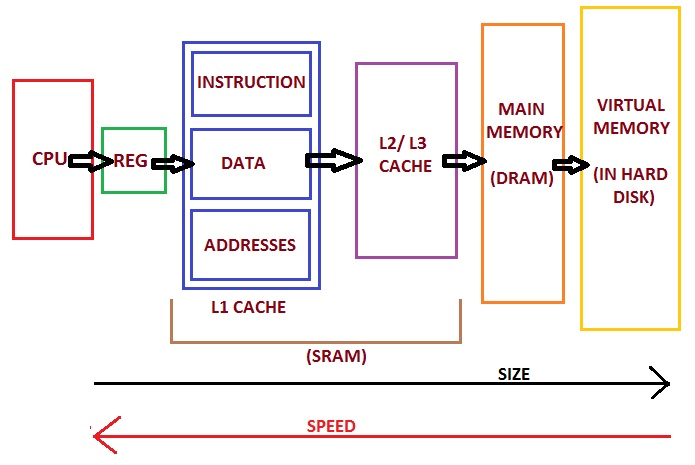
\includegraphics[width=.8\textwidth]{figures/CPU memory.jpg}
        \caption{Memory layout in the CPU}
        \label{fig:mem-cpu}
    \end{figure}
\end{frame}

\begin{frame}
    \frametitle{Background - Data oriented design}
    \begin{itemize}
        \item Difference struct and class: ability to hide data at compile time.
        \item Many repetitions of same pointer to functions: much wasted space.
        \item Therefore: Linear array of structs.
    \end{itemize}

    \begin{block}{Remark}
        *Array in the sense of CS, not C++
    \end{block}
\end{frame}

\end{document}
